\chapter{Network motifs}

It has been observed that, in most graphs that arise as models of real-world networks, like biological or social ones, some specific subgraph pattern may repeat consistently; these repeated patterns are called \emph{network motifs}, and  may be proper to a specifi network, or even shared among different ones. These subgraphs, defined by a particular pattern of interactions between the involved vertices, may reflect a behaviour for which particular functions are achieved efficiently. Indeed, motifs are of notable importance largely because they may reflect functional properties. Some purposes for exploiting network motifs are:
   \begin{itemize}
       \item Efficiency: to build better and/or faster algorithms;
       \item Classification: to find structural differences among graphs induced by different relations and measured counting the frequency of various motifs;
       \item Clustering: to analyze the structure of a graph based on the cuts induced by the motifs instead of those induced by the edges, this approach turns out to give the most satisfying results;
       \item Coordinate system: each motif instance may be viewed as a point in the space based on the number of motifs.
   \end{itemize}

   
\section{Triangles}

The triangle graph $\mathcal{K}_3$ is the simplest, nontrivial motif that is usually sought for. A specific coefficient is defined for it:
\begin{definition}[Global clustering coefficient]
    Let $G$ be a graph, where $G_\triangle$ contains all the subgraphs in $G$ that are triangles; define a \emph{connected triple} in $G$ as two edges of $G$ sharing a vertex $\{x, y\}, \{y, z\} \in E(G)$. Let $w(G)$ be the function that counts such connected triples in $G$. The \emph{global clustering coefficient} $c$ is a ratio of triangles over connected triples in $G$:
    \begin{equation}\label{eq:clustering-coefficient}
        c(G) = \frac{3 \abs{G_\triangle}}{w(G)}.
    \end{equation}
\end{definition}

The higher the coefficient, the more triangles the graph contains. An example of a graph along with its connected triples is swown in figure \ref{fig:graph-example-triangles}; note that when a triangle is present, there are three distinct connected triples, all sharing the same vertices but different edges. In total, there are $5$ connected triples and $1$ triangle, so the global clustering coefficient of the starting graph is $\frac{3}{5}$. If the specific case of a clique $\mathcal{K}_n$ is considered, then observe that all vertex triplets induce a triangle; in the end, $c(\mathcal{K}_n) = 1$.
\begin{figure}
    \centering
    
    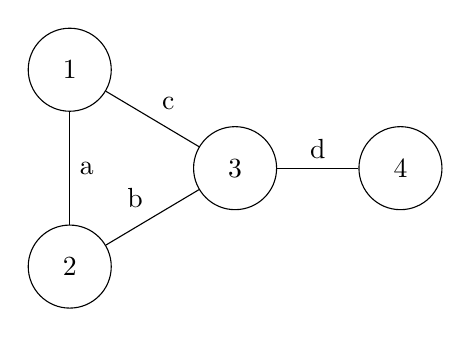
\begin{tikzpicture}[auto]
        \draw
            (0, 0) node (b) [draw, circle, minimum size = 3em] {$2$}
            (0, 2.5) node (a) [draw, circle, minimum size = 3em] {$1$}
            (2.1, 1.25) node (c) [draw, circle, minimum size = 3em] {$3$}
            (4.2, 1.25) node (d) [draw, circle, minimum size = 3em] {$4$}

            (a) edge node [midway] {a} (b)
            (a) edge node [midway] {c} (c)
            (b) edge node [midway] {b} (c)
            (c) edge node [midway] {d} (d)
        ;
    \end{tikzpicture}

    \vspace{7mm}

    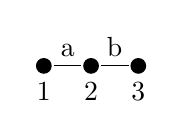
\begin{tikzpicture}
        \fill
            (0, 0) circle [radius = 1mm] node (a) {} node [below, outer sep = 1mm] {$1$}
            (0.6, 0) circle [radius = 1mm] node (b) {} node [below, outer sep = 1mm] {$2$}
            (1.2, 0) circle [radius = 1mm] node (c) {} node [below, outer sep = 1mm] {$3$}

            (a) edge node [midway, above] {a} (b)
            (b) edge node [midway, above] {b} (c)
        ;
    \end{tikzpicture}
    \hspace{8mm}
    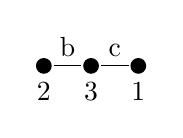
\begin{tikzpicture}
        \fill
            (0, 0) circle [radius = 1mm] node (a) {} node [below, outer sep = 1mm] {$2$}
            (0.6, 0) circle [radius = 1mm] node (b) {} node [below, outer sep = 1mm] {$3$}
            (1.2, 0) circle [radius = 1mm] node (c) {} node [below, outer sep = 1mm] {$1$}

            (a) edge node [midway, above] {b} (b)
            (b) edge node [midway, above] {c} (c)
        ;
    \end{tikzpicture}
    \hspace{8mm}
    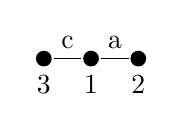
\begin{tikzpicture}
        \fill
            (0, 0) circle [radius = 1mm] node (a) {} node [below, outer sep = 1mm] {$3$}
            (0.6, 0) circle [radius = 1mm] node (b) {} node [below, outer sep = 1mm] {$1$}
            (1.2, 0) circle [radius = 1mm] node (c) {} node [below, outer sep = 1mm] {$2$}

            (a) edge node [midway, above] {c} (b)
            (b) edge node [midway, above] {a} (c)
        ;
    \end{tikzpicture}
    \hspace{8mm}
    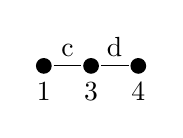
\begin{tikzpicture}
        \fill
            (0, 0) circle [radius = 1mm] node (a) {} node [below, outer sep = 1mm] {$1$}
            (0.6, 0) circle [radius = 1mm] node (b) {} node [below, outer sep = 1mm] {$3$}
            (1.2, 0) circle [radius = 1mm] node (c) {} node [below, outer sep = 1mm] {$4$}

            (a) edge node [midway, above] {c} (b)
            (b) edge node [midway, above] {d} (c)
        ;
    \end{tikzpicture}
    \hspace{8mm}
    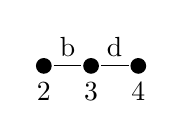
\begin{tikzpicture}
        \fill
            (0, 0) circle [radius = 1mm] node (a) {} node [below, outer sep = 1mm] {$2$}
            (0.6, 0) circle [radius = 1mm] node (b) {} node [below, outer sep = 1mm] {$3$}
            (1.2, 0) circle [radius = 1mm] node (c) {} node [below, outer sep = 1mm] {$4$}

            (a) edge node [midway, above] {b} (b)
            (b) edge node [midway, above] {d} (c)
        ;
    \end{tikzpicture}

    \caption{Example of a graph with its connected triples}
    \label{fig:graph-example-triangles}
\end{figure}

The next goal is to find a way to efficiently compute $c$. For starters, in order to compute $w$, a na\"ive way would be to count all possible neighbouring pairs of each vertex in $G$:
\[
	w(G) = \sum_{u \in V}\binom{deg(u)}{2}
\]

This idea drives the design of the algorithm in figure \ref{lst:triangles-alg1}:
\begin{lstlisting}[caption = {Algorithm 1}, label = {lst:triangles-alg1}]
Algorithm_1:
    $t \gets 0$   // the number of triangles
    for $u \in V$:
        for $\{ v, w \} \in \binom{N_u}{2}$:   // where $N_u$ is the set of the neighbors of $u$
            if $\{ v, w \} \in E$:
                $t = t + 1$
    return $\frac{t}{3}$
\end{lstlisting}

\begin{claim}\label{cl:triangles-1}
	Let $\abs{V} = n$. The algorithm in \ref{lst:triangles-alg1} has a time complexity in $O(n^3)$.
\end{claim}

\begin{proof}
    The outer loop iterates over all vertices, thus contributing a factor of $n$ to the loop body; the body itself consists of a nested loop over neighbouring doubletons, which in the worst case amount to $\oneover{2}(n - 1)(n - 2)$. The nested loop's body runs in constant time; therefore the total time complexity is:
    \[
        n \cdot \oneover{2}(n - 1)(n - 2) \in O(n^3)
    \]
\end{proof}

Observe that, in the event that the graph is sparse, the nested loop takes far less time, and the total running time tends to be linear in the extreme cases. Nevertheless, there are other algorithms that do improve time complexity for dense graphs.


\subsection{Adjacency Matrix method}

One algorithm to compute the number of triangles is based on the adjacency matrix multiplication. The adjacency matrix for a graph $G$ is the $n \times n$ matrix $A$ where each row and each column corresponds to a vertex in the graph, and for all matrix elements $a_ij$:
\[
    a_{ij} = \begin{cases}
        1 & \textsc{iff } \{i, j\} \in E(G) \\
        0 & \textsc{else}
    \end{cases}
\]

For example, here is the adjacency matrix of the graph in figure \ref{fig:graph-example-triangles}, along with its square:
\[
	A = \begin{pmatrix}
		0 & 1 & 1 & 0 \\
		1 & 0 & 1 & 0 \\
		1 & 1 & 0 & 1 \\
		0 & 0 & 1 & 0 \\
    \end{pmatrix}
    \qquad
	A^2 = \begin{pmatrix}
		2 & 1 & 1 & 1 \\
		1 & 2 & 1 & 1 \\
		1 & 1 & 3 & 0 \\
		1 & 1 & 0 & 1 \\
	\end{pmatrix}
\]

The squared matrix exhibits has a property that follows by matrix multiplication that is worth mentioning:
\[
	(A^2)_{uv} = \sum_{w \in G}A_{uw} \cdot A_{wv}
\]
where $A_{uw} = 1$ iff $u$ and $w$ are adjacent, and $A_{wv} = 1$ iff $w$ and $v$ are adjacent. Essentially, $(A^2)_{uv}$ expresses the number of $2$-paths of length going from $u$ to $w$; in the specific case of $A_{uu}$ there is the number of paths of length $2$ that go from $u$ to itself, which is equal to its degree because we can go from $u$ to any of its neighbours in $1$ step and then use the same edge to go back to $u$.

Going further with the cube, the formula for each element becomes:
\[
    (A^3)_{uv} = \left( A \cdot A^2 \right)_{uv} = \sum_{w \in G} A_{uw} \cdot (A^2)_{wv},
\]
which means, intuitively, that $(A^3)_{uv}$ contains the number of paths of length $3$ that go from $u$ to $v$; this reasoning generalizes to any $A^k$ for paths of length $k$.

Finding triangles in a graph then relies in computing the diagonal elements of $A^3$. For example, consider the graph $\mathcal{K}_3$ composed of a single triangle; starting from an arbitrary node $u$, there are indeed two paths of length $3$ that loop from $u$ to itself: $u \to v \to w$ and $u \to w \to v$. Therefore $(A^3)_{uu}$ would evaluate $2$, however the triangle is just one. That is true in general, so every triangle counts twice to the diagonal entry of every node that forms it; and since each node of the triangle detest it, said triangle does appear in $3$ differen diagonal entries, one for each vertex.

\begin{definition}
    Let $M$ be a matrix, its \emph{trace} is:
    \begin{equation}\label{eq:trace}
        tr(M) = \sum_i M_{ii}
    \end{equation}
\end{definition}

Thus the number of triangles can be expressed simply as:
\begin{equation} \label{eq:triangles-1}
	\abs{G_\triangle} = \frac{tr(A^3)}{6}
\end{equation}

This gives us the following algorithm, which receives a graph in form of it adjacency matrix, and performs the computations outlined above:
\begin{lstlisting}[caption = {Algorithm 2}, label = {lst:triangles-alg2}]
Algorithm_2(A):
    $AC \gets$ fast_mat_multiplication(A,3)
    return $\frac{tr(AC)}{6}$
\end{lstlisting}

Its running time is mainly governed by matrix multiplication, for which the best known algorithm takes time $O(n^{2.37})$. It entails that the time complexity is independent from the number of edges: in fact, the algorithm doesn't take into account the structure of the graph. On one hand, this approach gives an improvement for dense graphs, lowering the bound from $O(n^3)$ to $O(n^{2.37})$; but on the other hand it suffers a performance hit on sparse graphs. Note that this is true because, even if a matrix $A$ is sparse, its square $A^2$ won't. A good example showcasing this consequence is a star graph, for which the adjacency matrix on $7$ vertices and its square are:
\[
	A = \begin{pmatrix}
		0 & 0 & 0 & 0 & 0 & 1 & 0 \\
		0 & 0 & 0 & 0 & 0 & 1 & 0 \\
		0 & 0 & 0 & 0 & 0 & 1 & 0 \\
		0 & 0 & 0 & 0 & 0 & 1 & 0 \\
		0 & 0 & 0 & 0 & 0 & 1 & 0 \\
		1 & 1 & 1 & 1 & 1 & 0 & 1 \\
		0 & 0 & 0 & 0 & 0 & 1 & 0 \\
    \end{pmatrix}
    \qquad
	A^2 = \begin{pmatrix}
		1 & 1 & 1 & 1 & 1 & 0 & 1 \\
		1 & 1 & 1 & 1 & 1 & 0 & 1 \\
		1 & 1 & 1 & 1 & 1 & 0 & 1 \\
		1 & 1 & 1 & 1 & 1 & 0 & 1 \\
		1 & 1 & 1 & 1 & 1 & 0 & 1 \\
		0 & 0 & 0 & 0 & 0 & 6 & 0 \\
		1 & 1 & 1 & 1 & 1 & 0 & 1 \\
	\end{pmatrix}
\]


\subsection{Structure-based method}

Another approach to compute $c$ is driven from the observation that, by sorting the vertices by their degree and looking for triangles starting from vertices with lower degree, it is possible to avoid counting duplicates, and less checks are left to perform on higher degree vertices, since the lower ones are progressively excluded. The algorithm is shown in figure \ref{lst:triangles-alg3}.
\begin{lstlisting}[caption = {Algorithm 3}, label = {lst:triangles-alg3}]
Algorithm_3(G):
    $t \gets 0$
    $\pi \gets \sort(V, \min_{\deg})$
    $\forall i : 1 \to n$:
        $N \gets \{v \in \{\pi(i + 1), \dots, \pi(n)\} : \{\pi(i), v\} \in E(G)\}$       // Get all neighbours after current
        $\forall \{v, w\} \in \binom{N}{2}$:
            if $\{v, w\} \in E(G)$:
                $t \gets t + 1$
    return t
\end{lstlisting}

\begin{example}
    The ordering of the nodes of graph in figure [\ref{fig:graph-example-triangles}] is: \textit{4, 1, 2, 3}, since the degrees of the nodes are, respectively, \textit{1, 2, 2, 3}.
\end{example}

\begin{claim}\label{thm:triangles-2}
    The algorithm correctly computes $\abs{G_\triangle}$.
\end{claim}

\begin{proof}
    Each triangle is counted exactly once by the vertex that comes first in the permutation $\pi$.
\end{proof}

To start having an idea on what is the algorithm's running time, consider a clique $\mathcal{K}_n$; its edge count is tightly bounded by the square of the vertex count, and the maximum number of triangles that can be found is essentially $\abs{\powerset_3(V(\mathcal{K}_n))}$, which in turn has a tight bound on the cube of the vertex count. Therefore:
\[
    \left( m \in \Theta(n^2) \wedge \abs{(\mathcal{K}_n)_\triangle} \in \Theta(n^3) \right) \implies \abs{(\mathcal{K}_n)_\triangle} = \Theta(m^{3/2})
\]
This is true only if cliques are considered; the usual social graphs have much less edges in general, and better performances can thus be achieved.

\begin{theorem}\label{thm:triangles-3}
    Given $m = \abs{E(G)}$, the algorithm has a running time bound of $O(m^{\frac{3}{2}})$.
\end{theorem}

%\ex Let's consider the star again, with Algorithm\_3 we need only $O(n^{1.5})$, instead of $O(n^2)$.

%\obs Since we add at most 1 triangle at each step, there will be at most $O(\mathcal{E}^{3/2})$ triangles in the graph, furthermore \texttt{Algorithm\_3} [\ref{lst:triangles-alg3}] is able to return the whole list of triangles, along with their number.

\begin{proof}

    \begin{proposition}\label{prop:sqrte}
        For any graph $G = (V, E)$, where $\abs{V(G)} = n$ and $\abs{E(G)} = m$:
        \[
            \abs{\{v \in V(G) : \deg(v) \geq \sqrt{m}\}} \leq 2\ \sqrt{m}
        \]
    \end{proposition}
    \begin{proof}
        By absurd, if there are more vertices with such degree, the degree sum of them would be strictly greater than $\sqrt{m} \cdot 2 \sqrt{m} = 2 m$, which violates the degree sum property of graphs.
    \end{proof}
    
    Let $V_1$ and $V_2$ be a bipartition of $V(G)$ that separates the vertices with degree at least $\sqrt{m}$ from those that don't. Then, by using proposition [\ref{prop:sqrte}]:
    \[
        2 \abs{E(G)} = 2 m = \sum_{v \in V} \deg(v) \geq \sum_{v \in V_1} \sqrt{m} = \abs{V_1} \sqrt{m}
    \]

    The proof will mainly consist in counting exactly how many neighbouring pairs in total are checked by the algorithm; define this quantity as $P$:
    \[
        P = \sum_{i \in [n]} \abs{\binom{N^{(i)}}{2}} \leq \sum_{i \in [n]} \abs{N^{(i)}}^2
    \]

    \begin{lemma}\label{lem:triangles-1}

        \[
            \abs{N^{(i)}} \leq 2 \sqrt{m} \quad \forall \pi(i) \in V_1
        \]
    \end{lemma}
    \begin{proof}
        Remember that $\pi$ sorts the vertices by their degree; therefore the subsets $V_1$ and $V_2$ appear as two whole segments over $\pi$, $V_2$ coming first, and with $\sqrt{m}$ acting as a separator. Given a vertex $\pi(i) \in V_1$, since its neighbours are collected from $\pi(i + 1)$ afterwards, there cannot be more than $\abs{V_1} \leq 2 \sqrt{m}$ neighbours, therefore the lemma is proven.
    \end{proof}

    An upper bound for $T_1$ can now be formulated:
    \begin{equation}\label{eq:triangles-tv1}
        P_1 = \sum_{\substack{i \in [n] \\ \pi(i) \in V_1}} \abs{\binom{N^{(i)}}{2}} \leq \sum_{\substack{i \in [n] \\ \pi(i) \in V_1}} \abs{N^{(i)}}^2 \leq \sum_{\substack{i \in [n] \\ \pi(i) \in V_1}} \left( 2 \sqrt{m} \right)^2 \leq 8 m^{\frac{3}{2}}
    \end{equation}

    \todo{From here, things go downhill...}

    To give a similar bound to $T_2$, partition the vertices $v \in V_2$ in buckets $B_i$, such that:
    \[
        v \in B_i \iff \frac{\sqrt{m}}{2^i} \leq deg(v) < \frac{\sqrt{m}}{2^{i - 1}}
    \]

    By lemma [\ref{lem:triangles-1}] it entails that $\abs{B_1} \leq 4 \sqrt{m}$, consequently $\abs{B_2} \leq \frac{2 m}{\frac{\sqrt{m}}{4}} = 8 \sqrt{m}$, $\abs{B_3} \leq \frac{2 m}{\frac{\sqrt{m}}{8}} = 16 \sqrt{m}$, and so on. Thus, in general:
    \begin{equation}\label{lem:triangles-2}
        \abs{B_i} \leq 2^{i + 1} \sqrt{m}
    \end{equation}

    \begin{lemma}\label{lem:triangles-3}
        \begin{equation}\label{eq:triangles-tv2}
            P_2 = \sum_{u \in V_2} \abs{\binom{N_u^+}{2}} \leq \sum_{u \in V_2} \abs{N_u^+}^2 \leq \sum_{u \in V_2} deg(u)^2.
        \end{equation}
    \end{lemma}

    \begin{lemma}\label{lem:triangles-4}
        For $u \in V_2^{(i)}$, \texttt{algorithm-3} [\ref{lst:triangles-alg3}] does at most $m 2^{-2i}$ steps.
    \end{lemma}

    Putting together the upper bound for $P_2$ with the bound for $P_1$ shown in [\ref{eq:triangles-tv1}], a bound for $P$ is defined:
    \begin{align*}
        P_2 &= T_{V_2^{(1)}} + T_{V_2^{(2)}} + \ldots + T_{V_2^{(i)}} + \ldots + T_{V_2^{(k)}} & \\
        &= \sum_{i=1}^{\log_2 \sqrt{m}} \left( \abs{V_2^{(i)}} \cdot \left(\text{ work for } u \in V_2^{(i)} \right) \right) & \\
        &= \sum_{i=1}^{\log_2 \sqrt{m}} \left( 2^{i+2} \sqrt{m} \cdot m2^{-2i} \right) & \\
        &\leq m \sqrt{m} \cdot \sum_{i=1}^{\log_2 \sqrt{m}} 2^{-2i} \leq 4 m^{3/2} &
    \end{align*}
\end{proof}


\section{Motifs with more than three vertices}\label{sec:big-motifs}

Looking for motifs with more than three vertices becomes increasingly difficult as the motif's vertex count increases; in fact, the problem of counting the number of $k$-cliques in a graph for any $k$ is \np-complete. For this reason, approximations of the optimal solutions are sought for.

\begin{definition}
    Given a graph $G$ and a motif $H$ on $k$ vertices, let $c_H$ be the number of occurrences of the motif in $G$:
    \begin{equation}\label{eq:motif}
        c_H = \abs{\{U \subseteq V : G[U] \simeq H\}}
    \end{equation}
\end{definition}

The goal is to obtain an estimate $\hat{c}_H$ of $c_H$ such that $c_H - \varepsilon \leq \hat{c}_H \leq c_H + \varepsilon$ with probability $1 - p$.\footnote{Note that this is similar to the work done with the Randomized Pivot algorithm for Correlation clustering, see theorem [\ref{thm:clust-rp-approx}].} Since it would take an exponential amount of time to pick each subgraph of $k$ nodes and check if it is isomorphic to $H$, sampling is employed instead.
\begin{lstlisting}[caption = {Algorithm 1}, label = {lst:motifs-alg1}]
Algorithm_1(G, H):
    $U \pickUAR \binom{V}{k}$
    return $[G[U] \simeq H]$
\end{lstlisting}
Note that, to evaluate the truth of $[G[U] \simeq H]$, it takes only constant time, since we are considering only $k$ nodes, and so we'll need to verify at most $k!$ permutations of the nodes in $U$.

Because of its \uar{} nature, the expected value of the output of the algorithm is the ratio between the number of subgraphs of $G$ that are isomorphic to $H$ and the number of all $k$-subgraphs of $G$:
\begin{equation}\label{eq:eyh-1}
    E([G[U] \simeq H]) = \binom{\abs{V}}{k}^{-1} \sum_{\substack{F \leq G \\ F \simeq H}} 1 = \binom{n}{k}^{-1} c_H
\end{equation}

Such expectation is linear with respect to $c_H$, but we would like to obtain an unbiased estimator of $c_H$, i.e., a random variable $X_H$ such that $E[X_H] = c_H$. We can define it as follows:
\begin{equation}\label{eq:exh-1}
    X_H = \binom{n}{k} \cdot [G[U] \simeq H].
\end{equation}
In this way, the expected value is what we want, but the variance is very high: a single sample gives us 0 or $\binom{n}{k}$, nothing very useful, and we can't pick $\binom{n}{k}$ samples.

A possible improvement stems from the following observation. Since $H$ is connected, if we apply Algorithm 1 [\ref{lst:motifs-alg1}] on a sparse graph, we'll perform many useless samplings (we'll pick unconnected subgraphs with high probability). For example, the probability of picking a $k$-motif on a star is $k/n$. Thus, we can slightly modify the algorithm as follows:
\begin{lstlisting}[caption={Algorithm 1b}, label={lst:motifs-alg1b}]
Algorithm_1b(G, H):
    $U \pickUAR \binom{V}{k}$
    $F \gets G[U]$
    if $F$ is not connected:
        return "FAIL"
    else:
        return $[F \simeq H]$
\end{lstlisting}
But this doesn't produce a substantial improvement, so how can we pick $k$ nodes in such a way that they are connected, and that they have a high chance of forming the motif we are looking for? A possibility is to pick a random node, then choose one of its neighbors, then choose a neighbor of the selected neighbor, and so on. This idea is put to good use for a special case: the 3-star.


\subsection{4-motifs}

Let's consider different examples of motifs with 4 nodes, shown in figure [\ref{fig:4-motifs}]; among these variants, the 3-star has the unique property of not having any $4$-path inside of it. Considering the motifs from b. to f., if we use the procedure mentioned at the end of the previous section (sample a random node, choose one of its neighbors, choose a neighbor of the selected neighbor, and so on), they have different probabilities to be found, since they have a different number of 4-paths, increasing from b. to f.).

\begin{figure}
    \centering
    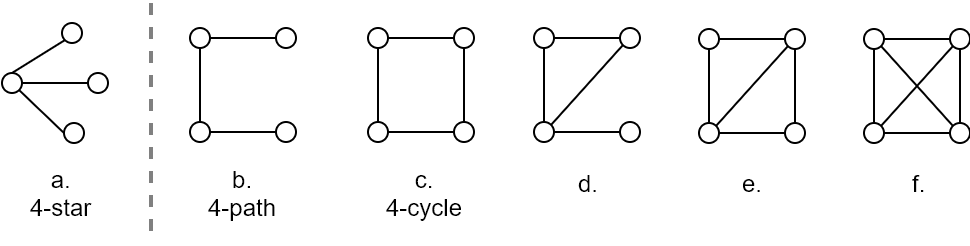
\includegraphics[width=0.9\textwidth]{4-motifs}
    \caption{Examples of 4-motifs}
    \label{fig:4-motifs}
\end{figure}

Let's describe an algorithm for finding 4-paths (b.) in a graph:
\begin{lstlisting}[caption={Algorithm 2 (Path sample)}, label={lst:motifs-alg2}]
Path sample(G):
    $u_1 \pickUAR V$
    $\forall i : (2, 3, 4)$:
        $u_i \pickUAR {v : \{u_{i - 1}, v\} \in E(G)}$
    return $Y_H = [G[\{u_1, u_2, u_3, u_4\}] \simeq H]$;
\end{lstlisting}

Let's study the expected value of the result of \texttt{Path sample}. Note that the algorithm can pick the path $u_1 \to u_1 \to u_2 \to u_3 \to u_4$ or the path $u_4 \to u_3 \to u_2 \to u_1$. Then:
\begin{align*}
    E(Y_H) &= \sum_{\substack{F \leq G \\ F \simeq H}} \Pr[u_1, u_2, u_3, u_4 \in V(F)]                                                                 & \\
    &= \sum_{\substack{F \leq G \\ F \simeq H}} \left( \oneover{n} \cdot \oneover{\deg(u_1)} \cdot \oneover{\deg(u_2)} \cdot \oneover{\deg(u_3)} + \oneover{n} \cdot \oneover{\deg(u_4)} \cdot \oneover{\deg(u_3)} \cdot \oneover{\deg(u_2)} \right) & \\
    &= \sum_{\substack{F \leq G \\ F \simeq H}} \oneover{n \cdot \deg(u_2) \cdot \deg(u_3)} \left( \oneover{\deg(u_1)} + \oneover{\deg(u_4)} \right)    & \\
    &= \sum_{\substack{F \leq G \\ F \simeq H}} \sigma_F                                                                                                &
\end{align*}

\todo{Not sure if this and the rest is right, applying something specific to F to a generic formula on H feels very wrong}

While the probability of hitting any node in \texttt{Algorithm 1} [\ref{lst:motifs-alg1}] was uniform, thus yielding a sum of the same value for each $F$, the probability of sampling a node in \texttt{Path sample} [\ref{lst:motifs-alg2}] depends on the degrees of the vertices previously picked, except for the first one. The consequence of this is that some 4-paths become easier to find than others; for example an isolated 4-path, where each node has degree $1$ or $2$, has higher probability of being detected than most other 4-paths.

To obtain an expected value of $c_H$, this bias has to be addressed, so we apply a compensation factor to $Y_H$, similarly to what we did in [\ref{eq:exh-1}]:
\begin{equation}\label{eq:exh-2}
    X_H = \frac{1}{\sigma_F} \cdot Y_H.
\end{equation}

Let $Y_F$ be a random variable that, given a subgraph $F$, its nodes are picked by the algorithm with probability $p$, and $X_F := Y_F \cdot \frac{1}{\sigma_F}$, then
\begin{align*}
          \variance(X_F)
       =&\ \variance \left( Y_F \cdot \oneover{\sigma_F} \right)    & \\
       =&\ \frac{\variance(Y_F)}{\sigma_F^2}                        & \\
       =&\ \frac{\sigma_F (1 - \sigma_F)}{\sigma_F^2}               & \\
       =&\ \frac{1 - \sigma_F}{\sigma_F}                            & \\
       =&\ \frac{1}{\sigma_F} - 1                                   & \\
    \leq&\ \oneover{\sigma_F} \in O\left(n\Delta^3\right)    &
\end{align*}
where $\Delta$ is the maximum degree of the graph. Thus, if the graph is sparse, $\variance(X_F) = O(n)$.

At this point, it's important to note that there is a problem in the algorithm [\ref{lst:motifs-alg2}]: when a node $u_i$ is picked, along with a neighbour $u_{i + 1}$, it is possible that when picking $u_{i + 2}$, $u_i$ is picked again, defeating the search for 4-paths. However, this problem can be solved in simple ways; for example by backtracking to the second step of the algorithm if $F$ does not contain 4 nodes.

\texttt{Path sample} is an example of a \emph{rejection sampling} algorithm: it picks new elements at random and increments a counter if they match some criterion, otherwise the elements are thrown away. A strength of the algorithm is that it actually produces the list of the motifs it finds, not just their number. This behavior is similar to that of \texttt{Algorithm 3} for triangles [\ref{lst:triangles-alg3}] but opposite to that of \texttt{Algorithm 2} for triangles [\ref{lst:triangles-alg2}].  For other kind of motifs, the same algorithm can be used, but the probability $\sigma_F$ will change.